\title{Final Exam for Algebra-Based Physics-1: Mechanics (PHYS135A-01)}
\author{Dr. Jordan Hanson - Whittier College Dept. of Physics and Astronomy}
\date{December 13th, 2017}
\documentclass[10pt]{article}
\usepackage[a4paper, total={18cm, 27cm}]{geometry}
\usepackage{outlines}
\usepackage[sfdefault]{FiraSans}
\usepackage{graphicx}

\begin{document}
\maketitle

\section{Conceptual Questions}
\subsection{Kinematics and Angular Kinematics}
\begin{enumerate}
\item If an object is dropped, it accelerates downward at $g$ m/s$^2$ (no air resistance).  If it is \textit{thrown} downward, the acceleration downward
\begin{itemize}
\item is less than $g$
\item is more than $g$
\item remains $g$
\end{itemize}
\item If an object is released from an aircraft moving at constant velocity (no air resistance), it accelerates downward, but travels along with the aircraft horizontally.  An observer from the ground observes the object
\begin{itemize}
\item traveling in a curved trajectory downward
\item traveling in a straight but diagonal trajectory forward
\item traveling straight downward
\item traveling in a straight but diagonal trajectory backward
\end{itemize}
\item An object accelerates with constant acceleration.  The displacement versus time curve is quadratic.  The velocity versus time plot should be $\rule{1cm}{0.15mm}$ and the acceleration versus time plot should be $\rule{1cm}{0.15mm}$.
\begin{itemize}
\item quadratic, linear
\item linear, flat
\item flat, linear
\item linear, quadratic
\end{itemize}
\item A potter spins clay on a wheel, making a vase.  She begins with an upright cylinder that spins at constant angular velocity.  After squeezing the clay, the radius of the cylinder shrinks.  What happens to the velocity of a point along the edge of the cylinder, if the angular velocity remains the same?
\begin{itemize}
\item It increases.
\item It remains the same.
\item It decreases.
\item Depends on the initial and final radius.
\end{itemize}
\item A battleship fires simultaneously two shells at enemy ships (Fig. \ref{fig:battle}).  If the shells follow the parabolic trajectories shown, which ship gets hit first?
\begin{itemize}
\item A
\item Both at the same time
\item B
\end{itemize}
\begin{figure}[hb]
\centering
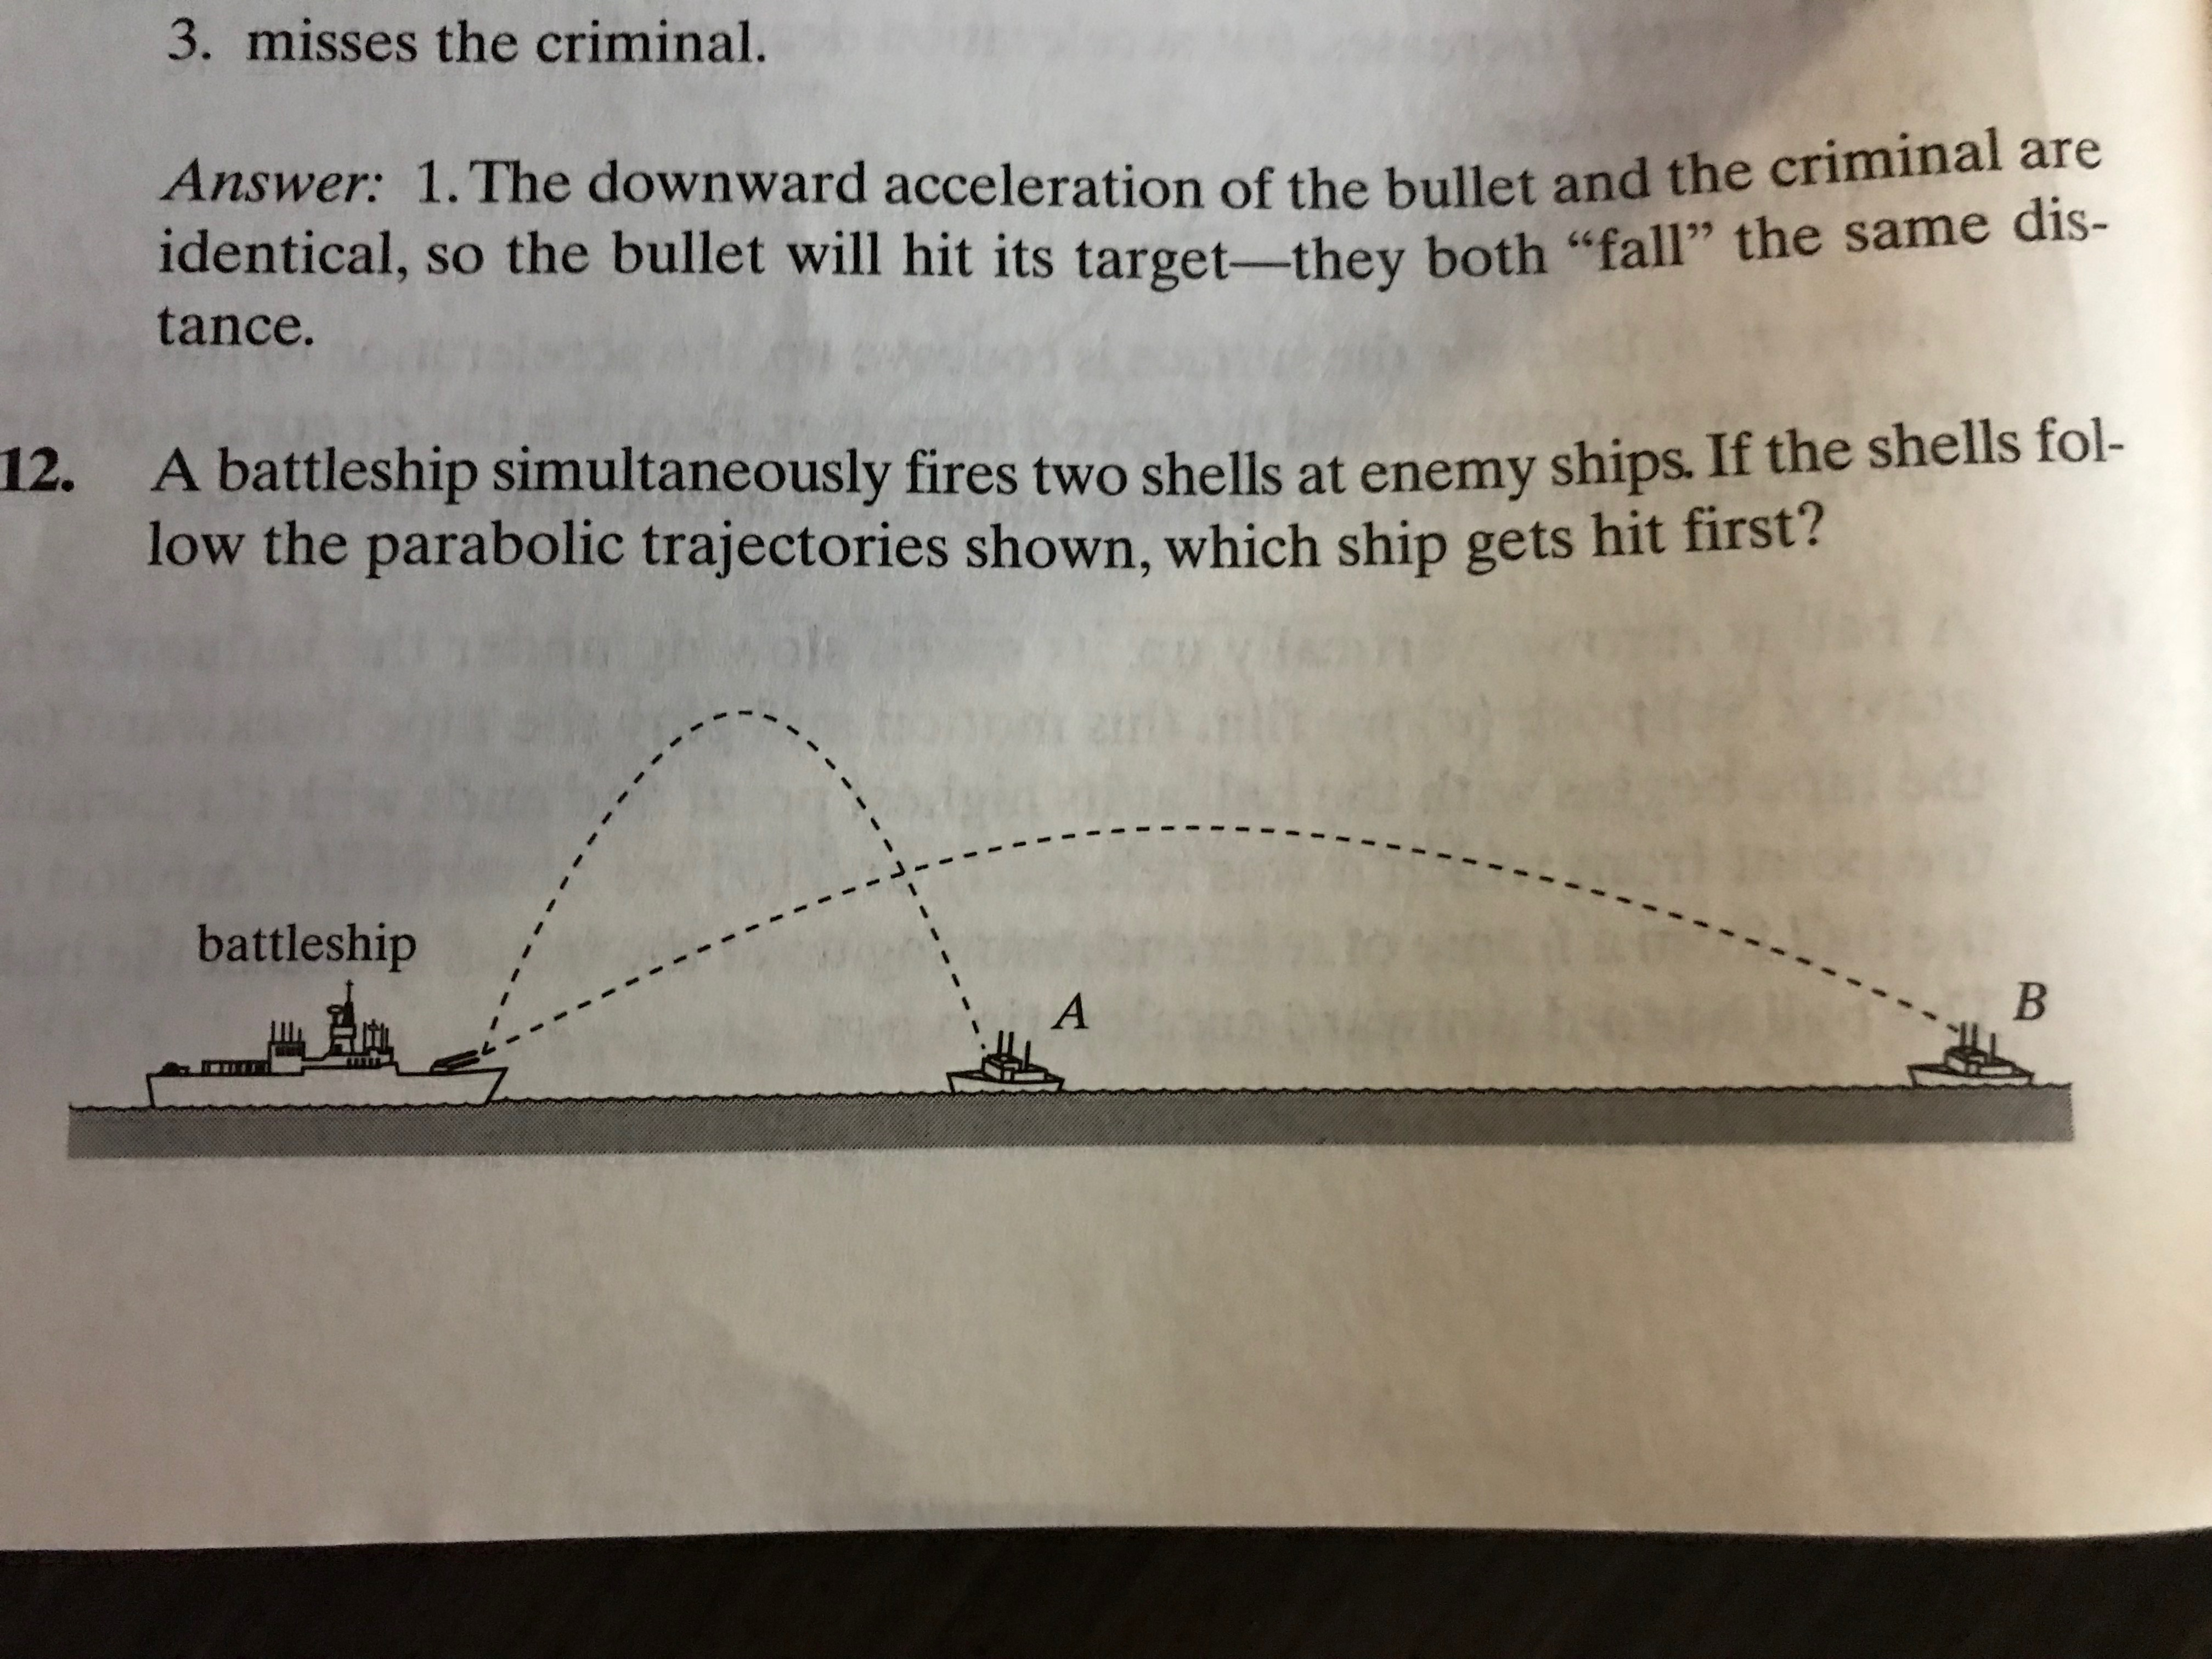
\includegraphics[width=0.6\textwidth,trim=0cm 30cm 0cm 45cm,clip=true]{battle.jpeg}
\caption{\label{fig:battle} Which ship is hit first?}
\end{figure}
\end{enumerate}
\subsection{Forces and Torque}
\begin{enumerate}
\item An elevator contains a person standing on a scale.  The elevator accelerates upward, then moves at constant velocity, then decelerates to a stop.  The scale reads a weight that is $\rule{1cm}{0.15mm}$, then $\rule{1cm}{0.15mm}$, and then $\rule{1cm}{0.15mm}$ the person's actual weight.
\begin{itemize}
\item More than, equal to, less than
\item Less than, equal to, more than
\item equal to, equal to, equal to
\item More than, equal to, equal to
\end{itemize}
\item A crate is pushed across a floor at constant velocity against friction.  If the crate is flipped so that a side with less surface area is on the bottom, and pushed again at constant velocity, the required force is
\begin{itemize}
\item More than the first side
\item Less than the first side
\item Equal to the first side
\end{itemize}
\item A man needs to pull a rusty lever to release a mechanism, but he can't.  His best bet is to
\begin{itemize}
\item Tie a rope to the lever, and pull on the rope in the same direction.  This will increase torque.
\item Bolt a metal rod to the level, and pull on the end of the rod.  This will increase torque.
\item Suspend his whole weight on the lever by hanging from it with one hand.  This will maximize torque.
\end{itemize}
\item A Formula 1 racecar makes a turn at constant velocity, and the road is flat.  There is friction between the road and tires.  Which of the following is true?
\begin{itemize}
\item The car experiences centripetal acceleration, provided by friction.
\item The car experiences centripetal acceleration, provided by the normal force.
\item Moving at constant velocity, the car experiences no acceleration.
\end{itemize}
\end{enumerate}
\subsection{Work and Energy}
\begin{enumerate}
\item In which of the follow situations would energy \textit{not} be conserved?
\begin{itemize}
\item An object is dropped from some height and experiences free-fall, neglecting air-resistance.
\item An oscillator is compressed by mass for a given displacement and then the mass is released.
\item A pendelum is pulled away from equilibrium and then released.
\item A rock slowly skids to a stop on top of a frozen pond.
\end{itemize}
\item A ball rolls down a hill that has a height $h$, attaining a speed $v$ at the bottom.  In order to attain a speed of $2v$ at the bottom, how tall would the hill have to be?
\begin{itemize}
\item $2h$
\item $3h$
\item $4h$
\end{itemize}
\end{enumerate}
\subsection{Linear and Angular Momentum}
\begin{enumerate}
\item A mine cart is moving along a track at constant speed, and passes under a vertical waterfall.  Because the cart is filled with water, the speed of the cart
\begin{itemize}
\item increases
\item decreases
\item remains constant (no net forces)
\end{itemize}
\item If ball 1 in the arrangement shown in Fig. \ref{fig:newton} is pulled back and then let go, ball 5 bounces forward.  If balls 1 and 2 are pulled back and released, balls 4 and 5 bounce forward, and so on.  The number of balls bouncing on each side is equal because
\begin{itemize}
\item of conservation of momentum.
\item the collisions are elastic.
\item neither of the above.
\end{itemize}
\begin{figure}
\centering
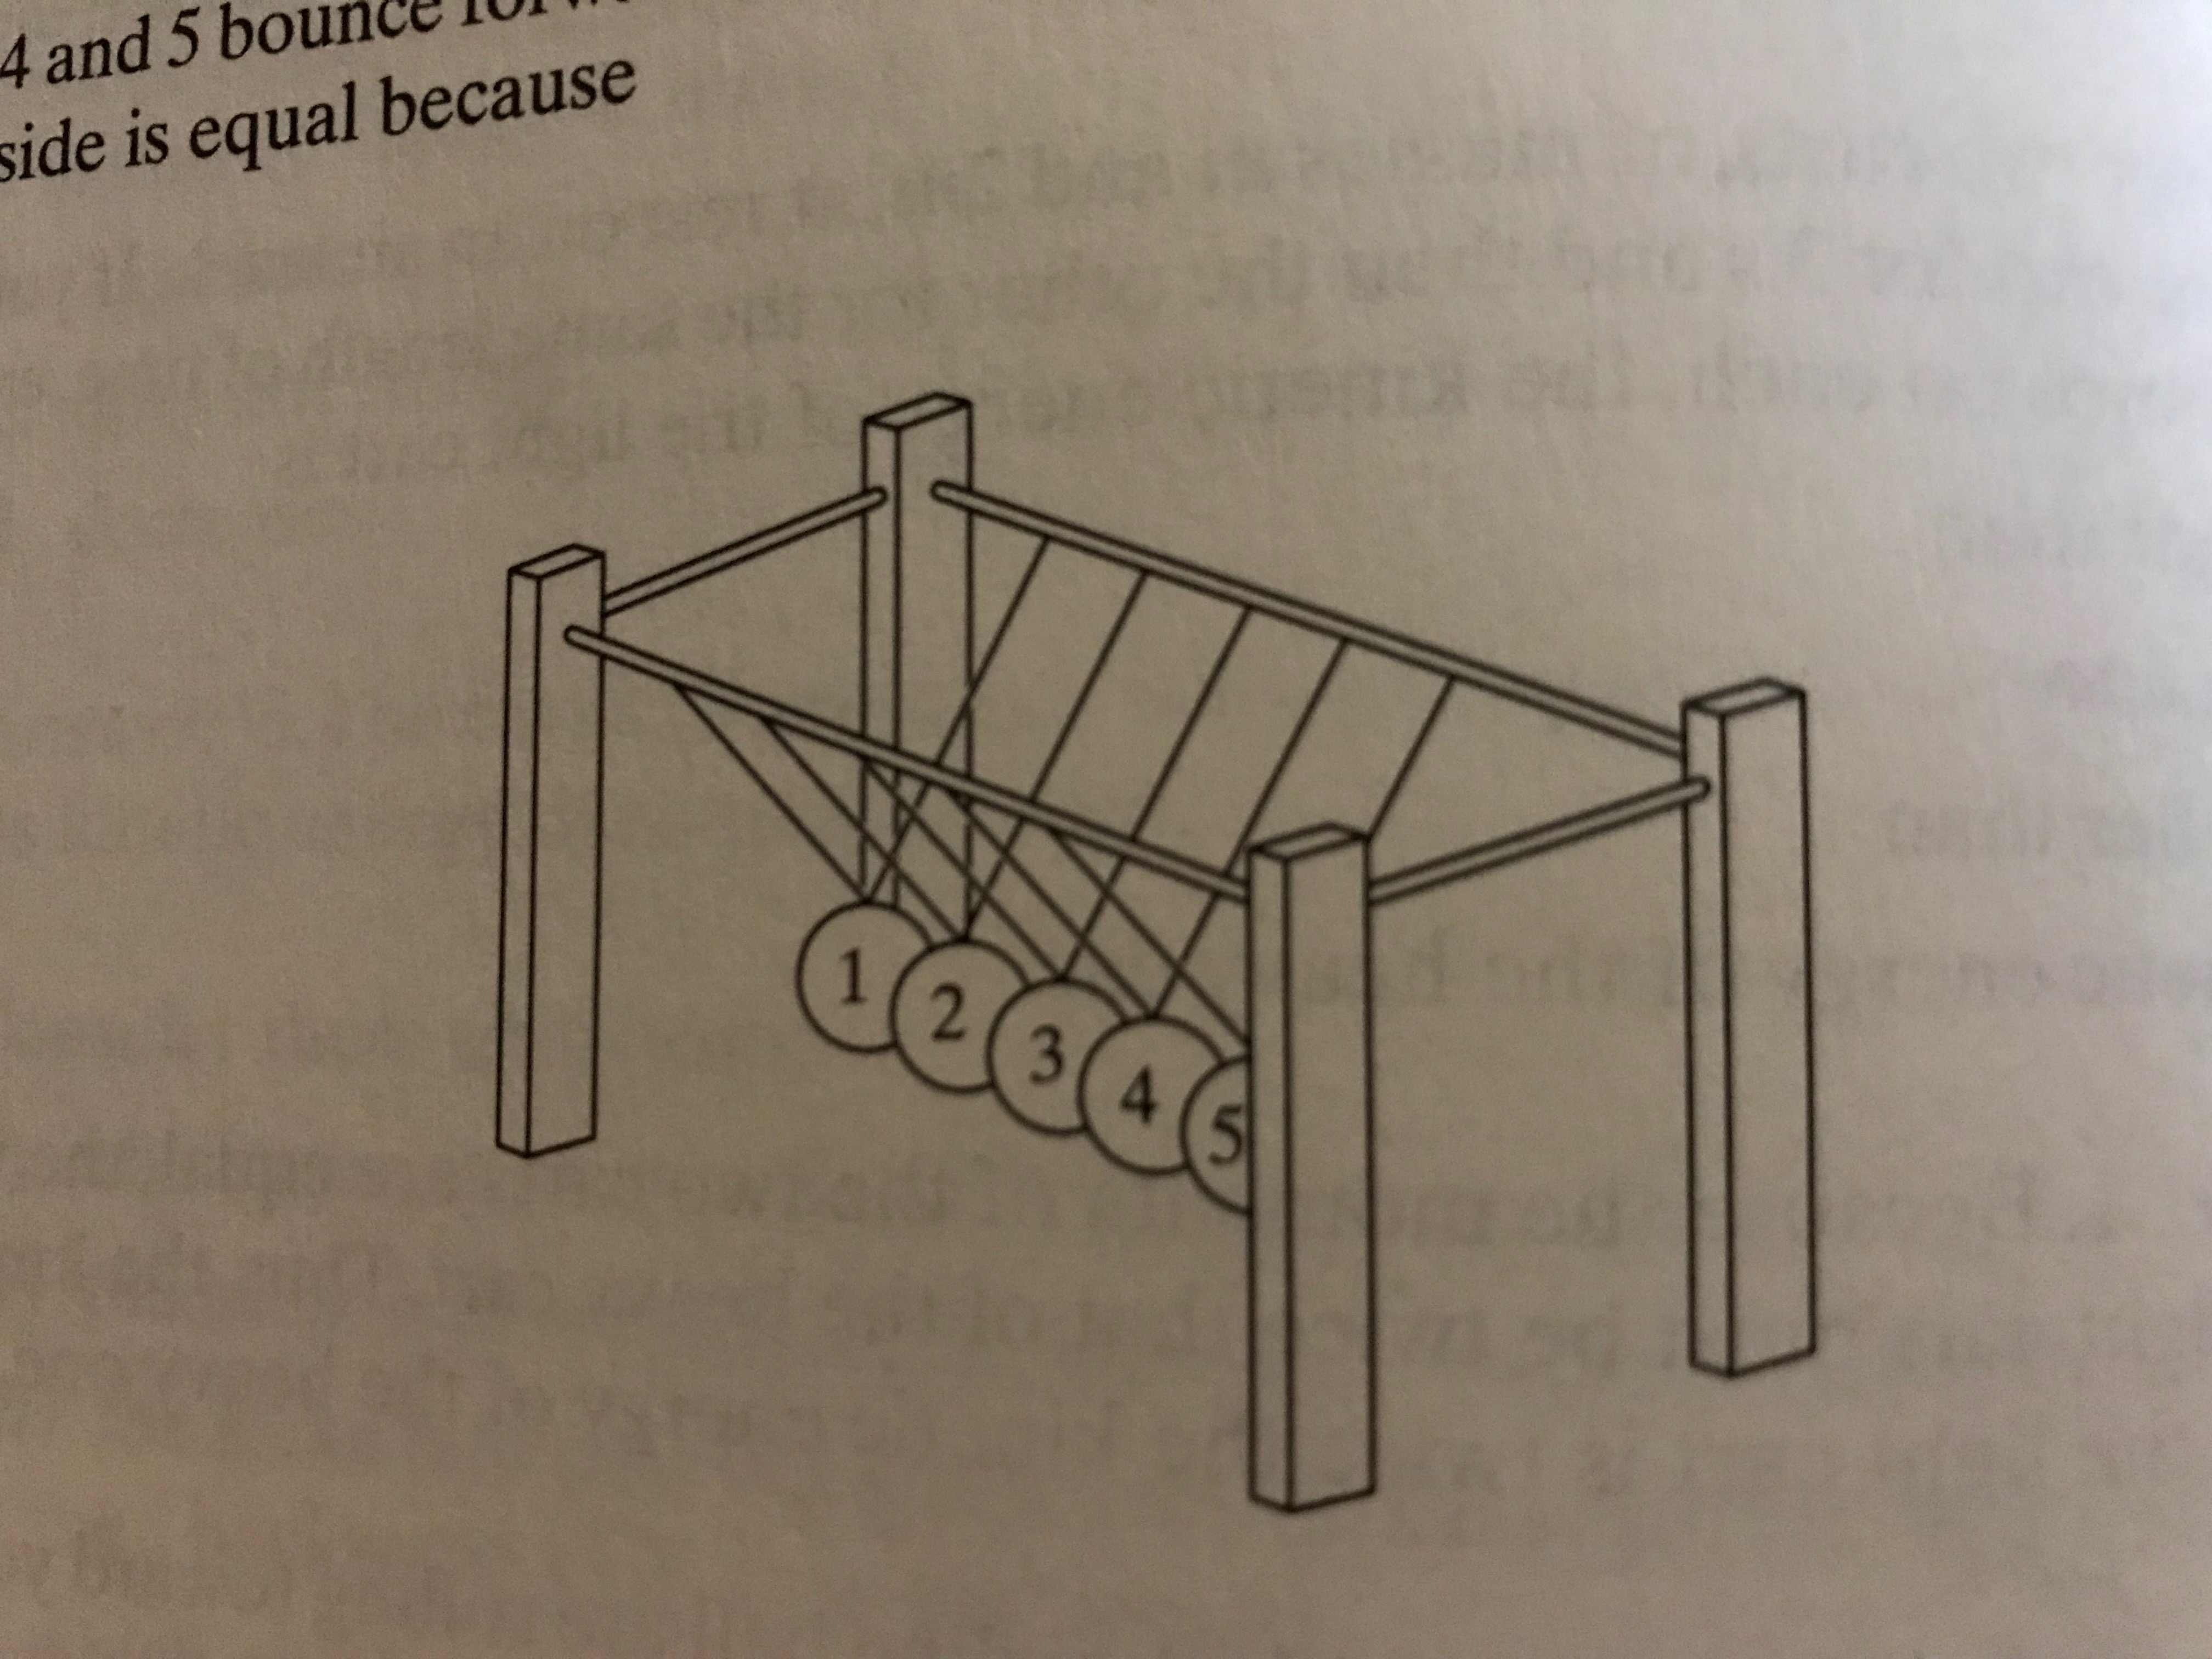
\includegraphics[width=0.3\textwidth,trim=20cm 5cm 15cm 20cm,clip=true]{newton.jpeg}
\caption{\label{fig:newton} This object is known as a Newton's cradle.}
\end{figure}
\item A star undergoes a supernova, in which significant matter is blown away by a fusion reaction.  The star also shrinks in size.  Suppose the radius decreases by a factor of 100.  By what factor does the angular velocity increase, if angular momentum is conserved?
\begin{itemize}
\item 10$^2$
\item 10$^3$
\item 10$^4$
\end{itemize}
\end{enumerate}
\section{Technical Questions}
\subsection{Kinematics and Angular Kinematics}
\begin{enumerate}
\item Question 
\end{enumerate}
\subsection{Forces and Torque}
\begin{enumerate}
\item Question
\end{enumerate}
\subsection{Work and Energy}
\begin{enumerate}
\item Question
\end{enumerate}
\subsection{Linear and Angular Momentum}
\begin{enumerate}
\item Question
\end{enumerate}
\end{document}